\documentclass[problem]{mcs}

\begin{pcomments}
  \pcomment{MQ_matching_afternoon}
  \pcomment{by Peter (Jian) Huang 10/27/11, minor edit by ARM}
\end{pcomments}

\pkeywords{
  matching
  bipartite
  bottleneck
}

%%%%%%%%%%%%%%%%%%%%%%%%%%%%%%%%%%%%%%%%%%%%%%%%%%%%%%%%%%%%%%%%%%%%%
% Problem starts here
%%%%%%%%%%%%%%%%%%%%%%%%%%%%%%%%%%%%%%%%%%%%%%%%%%%%%%%%%%%%%%%%%%%%%

\begin{problem}
Explain why the graph $G$ below
\iffalse
\idx{bipartite graph} $G$ in
Figure~\ref{fig:bipartite_with_bneck} \fi
has no \idx{matching}.

%\hint Looking at the graph from right to left may be easier.

\iffalse
Consider the bipartite graph $G$ in
Figure~\ref{fig:bipartite_with_bneck}. Explain why there is no
matching that covers $L(G)$? \\ (Hint: Hall's Theorem.  Also looking at
the graph from right to left may be easier)
\fi

\begin{center}
%\begin{figure}%\inhandout{[h]}
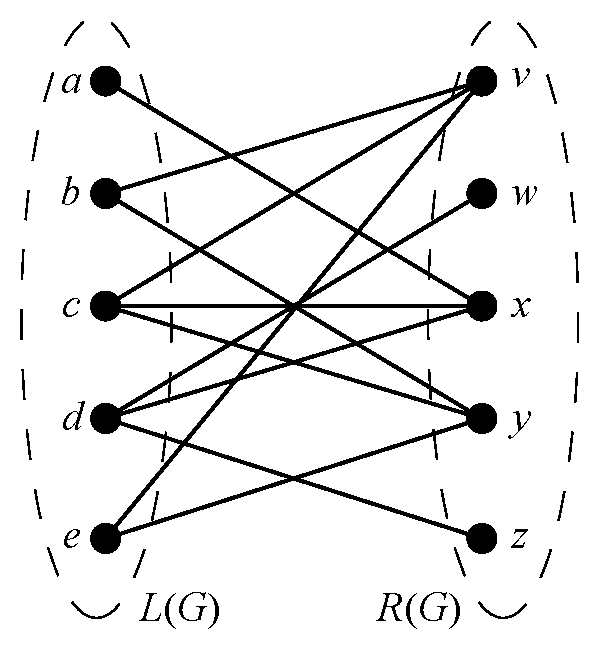
\includegraphics[width=2.2in]{MQ_bipartite_with_bottleneck}
%\caption{graph $G$.}
%\label{fig:bipartite_with_bneck}
%\end{figure}
\end{center}

\begin{solution}
It is not possible because $\set{a,b,c,e}$ is a bottleneck:
$\card{\edges{G}(\set{a,b,c,e})} = \card{\set{v,x,y}} = 3 < 4 =
\card{\set{a,b,c,e}}$.

Since the left and right vertex sets of $G$ are the same size, there
is a bottleneck on the right iff there is one on the left.  So an
alternative answer is to observe that $\set{w,z}$ is a bottleneck in
the other direction: $\card{\edges{G}^{-1}(\set{w,z})} = \card{\set{d}} = 1 <
2 = \card{\set{w,z}}$.

\end{solution}

\examspace

\end{problem}

\endinput
